\newpage
\section{Prinsipiell løsning}
\label{prinsipiellLoesning}

\subsection{Kretstopologi}
\label{kretstopologi}

En differensialforsterker er en nøkkelkomponent i designet av operasjonsforsterkere (op-amp)\cite[s. 105]{Art of Eletronics}. I en differensialforsterker benyttes ofte to inngangstransistorer i en konfigurasjon som tillater differensiell signalbehandling. Bipolare transistorer, som for eksempel NPN- og PNP-transistorer, er valgt for deres egenskaper som forsterkningsenheter og deres evne til å drive signaler med høy presisjon. Et typisk eksempel på en differensialforsterker er vist i figur \autoref{fig:diffamp}.

\begin{figure}[h]
    \centering
    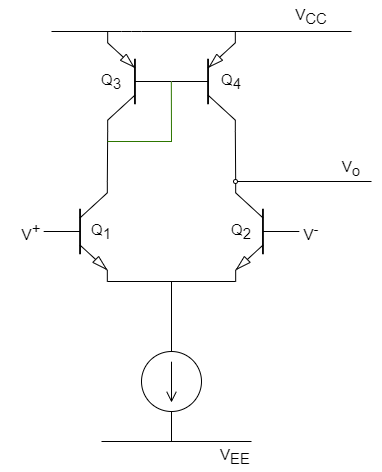
\includegraphics[width=0.6\textwidth]{Bilder/diffamp.drawio.png}
    \caption{Differensialforsterker som en operasjonsforsterker}
    \label{fig:diffamp}
\end{figure}


\subsection{Forsterkning}
\label{forsterkning}
For å finne forsterkningen til en op-amp, kan man gå utifra \autoref{eq:opamp} og omformulere den til \autoref{eq:forsterking}. Her er $V^+$ og $V^-$ spenningen inn på den positive og negative inngangen til opampen (Differnasnen mellom de vil bli omtalt som $V_{in}$). $V_{o}$ er spenningen ut av opampen over lasten og da blir $A$ forsterkningen til opampen.
\begin{equation}
    A = \frac{V_{o}}{(V^+ - V^-)} = \frac{V_{o}}{V_{in}}
    \label{eq:forsterking}
\end{equation}


\subsection{Total harmonisk distorsjon}
\label{totalHarmoniskDistorsjon}

Total harmmonisk distorsjon er hvor mye av det orginale signalet dominerer over harmoniske multiplikkative versjoner av seg selv, og er en vanelig måleenhet for støymåling i et ikke linjeært system. Man benytter seg av $V_{RMS}$ på både den orgainale frekvensen og på alle harmoniske frekvenser. For å finne total harmonisk distorsjon, kan vi bruke \autoref{eq:THD}. Her er $V_{1}$ er er spenningen ut av opampen ved en sinusformet inngangsspenning og $V_n$ RMS verdien til den n'te harmoniske frekvensen.

\begin{equation}
    THD(\%) = \frac {\sqrt {V_2^2 + V_3^2 +V_4^2 + \ldots + V_n^2}}{V_1} \cdot 100
    \label{eq:THD}
\end{equation}



\textbf{velg en av de to under, sjekk formelen}


\subsection{Åpen Løkke forsterkning}
\label{aapenLoekkeForsterkning}

For å beregne åpen løkke forsterkning, kan følgende ligning \autoref{eq:aapenLoekkeForsterkning} benyttes. Her representerer $V_{out}$ utgangsspenningen fra opampen. $V_{in}$ er inngangsspenningen til opampen, og $A$ er forsterkningen til opampen. Åpen løkke betyr at det ikke er noen tilbakekobling i kretsen \cite{Eletronics}.

\begin{equation}
    V_{out} = AV_{in}
    \label{eq:aapenLoekkeForsterkning}
\end{equation}

